\chapter{Identify project and Mission statement \\
% \small{\textit{-- Ashay Pable}} 
%\index{Chapter!Homework One -- Requirements}
\index{Identify project and Mission statement}
\label{Chapter::Identify project and Mission statement}}

% Add a section and label it so that we can reference it later
\section{Team Members \label{Section::teamMembers}}
\begin{enumerate}
  \item \textbf{Ashay Pable} : I am a Masters in Software Engineering student. I have worked as a software
developer for 4 years in India with a wide range of experience from Artificial Intelligence to
3D Graphics development. I have a keen interest in automation powered by AI and research
in contributing fields. My experience as a developer has made me realise the importance of
planning and documentation before initiation of a project
  \item \textbf{Divyamshu Mandadi} : My name is Divyamshu Mandadi and I’m currently in my third
semester doing my Masters in Software Engineering. Before moving to the US I have
worked as a Software Developer in India. My experience while working there combined
with the curiosity to learn more about the Software development processes led me here.
  \item \textbf{Neel Savani} : My name is Neel Savani. I had completed my under-graduation in Informa-
tion and Technology at birla vishwakarma mahavidhyalaya. I am currently in my second-
semester pursuing my masters in Software engineering. I am interested in developing soft-
ware.
\end{enumerate}

\section{Team Name \label{Section::teamName}}
"Group 3 - Inventory Management System for Retail Stores"
\section{Project Chosen \label{Section::projectChosen}}
\begin{itemize}
 \item Inventory Management system for Retail Stores.
 \item The project's goal is to create an intuitive and efficient inventory management system that will provide a retail business with real-time visibility into inventory levels and movement.
\end{itemize}
\section{Project Mission Statement \label{Section::projectMissionStatement}}
Our mission is to provide seamless and continuous supply of inventory so that customers needs are catered to in an efficient manner. Our system will provide an intuitive user interface that enables efficient recording and management of each item in the inventory. Retailers will be able to minimize stockouts, manage inventory levels for maximum profitability, and base data-driven choices on real-time inventory levels. This system provides a comprehensive solution that improves inventory management for retail establishments, frees up time, reduces expenses, and increases overall operational performance.

% \cite{GM1998}.

%\begin{figure}
%\centering
%\scalebox{0.8}{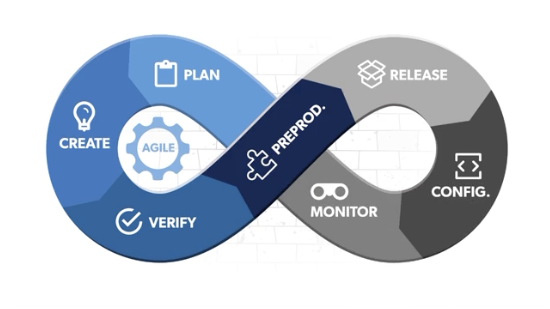
\includegraphics{Figures/manAgileProcess.png}}
%\caption{\label{Figure::manAgile} Figure of the continuous agile process.}
%\end{figure}

% add a new page
\newpage
